%% !TEX root = ../Thesis.tex
%% !TEX output_directory
\documentclass[11pt,a4paper,english,greek,twoside]{../Thesis}
%\usepackage[T1]{fontenc}
%\usepackage{algorithm, algpseudocode}% http://ctan.org/pkg/algorithmicx
%\usepackage{amsmath}



\begin{document}
\chapter{Κατάτμηση Δράσεων}
Η κατάτμηση ενός βίντεο δράσεων είναι απλά ο διαχωρισμός του σε τμήματα στα οποία συμβαίνει μόνο μία δράση. Οι βασικές προσεγγίσεις κατάτμησης στηρίζονται είτε σε επιβλεπόμενες είτε σε μη επιβλεπόμενες είτε σε ημιεπιβλεπόμενες μεθόδους μάθησης. Η πρώτη κατηγορία αξιοποιεί μοντέλα δράσεων και σύμφωνα με αυτά επιχειρεί να λύσει το πρόβλημα της κατάτμησης ως ένα πρόβλημα βελτιστοποίησης πάνω στα σκορ βεβαιότητας για κάθε θραύσμα. Οι μη επιβλεπόμενες μέθοδοι συνήθως στηρίζονται στις ομοιότητες μιας οικογένειας βίντεο προκειμένου να αποφασίσουν για τα όρια μιας δράσης που επαναλαμβάνεται σε όλα τα βίντεο. Τέλος, οι ημιεπιβλεπόμενες μέθοδοι επιχειρούν να σπάσουν το βίντεο σε συμπαγή κομμάτια έχοντας σαν οδηγό ένα αρχείο κειμένου. Οι δύο τελευταίες περιπτώσεις μπορούν να οδηγήσουν και στην αυτόματη εξαγωγή αναπαράστασης για τη δράση. Σε αυτή την εργασία εφαρμόζουμε τεχνικές επιβλεπόμενης μάθησης, οπότε θα εστιάσουμε σε αναφορές σε αυτές. Παρόλα αυτά, θα δοθούν και κάποια ενδιαφέροντα παραδείγματα που αξιοποιούν οποιαδήποτε από τις άλλες δύο μεθόδους επίσης.


\section{Ιδέες και Τεχνικές Κατάτμησης Βίντεο}
Πολλές εργασίες επιχείρησαν να προσεγγίσουν μαθηματικά το πρόβλημα καταλήγοντας σε ένα πρόβλημα βελτιστοποίησης. Το \cite{lv_2006} προσεγγίζει το ζήτημα με κρυφά μαρκοβιανά μοντέλα που ενσωματώνουν τη δυναμική των δράσεων και χρησιμοποιεί τον ταξινομητή AdaBoost για την τελική απόφαση. Το \cite{shi_2008} εφαρμόζει ημιμαρκοβιανά μοντέλα λαμβάνοντας υπόψιν χαρακτηριστικά εντός των τμημάτων αλλά και στα σύνορα αυτών με τα γειτονικά τμήματα, ενώ η αναπαράσταση των γειτονικών τμημάτων επηρεάζει το τρέχον τμήμα. Το πρόβλημα ελαχιστοποίησης επιλύεται με έναν αλγόριθμο τύπου Viterbi. Στο \cite{bargi_2012} συνδυάζονται κρυφά μαρκοβιανά μοντέλα με ιεραρχικές διαδικασίες Dirichlet επιλύοντας πρόβλημα κατάτμησης με άγνωστο αριθμό κλάσεων. Το \cite{kosmopoulos_2014} λαμβάνει υπόψιν τον μετασχηματισμό Hough για την δημιουργία προτάσεων ορίων θραυσμάτων. Ένας ταξινομητής SVM χρησιμοποιείται για να αποδώσει σκορ στα θραύσματα και η βέλτιστη κατάτμηση επιτυγχάνεται με χρήση δυναμικού προγραμματισμού. Η μέθοδος αυτή είναι λειτουργική ακόμα και σε περιπτώσεις όπου υπάρχουν άγνωστες κλάσεις.

\par Άλλες εργασίες δίνουν έμφαση στο είδος των χαρακτηριστικών που διακρίνουν τα τμήματα μεταξύ τους. Το \cite{jiang_2012} χρησιμοποιεί χαρακτηριστικά HOG και οπτικής ροής για να εξάγει μοντέλα για κάθε frame. Αφού ταξινομήσει κάθε frame ξεχωριστά, αθροίζει τις πιθανότητες των frames για να εξάγει την δράση. Η ταξινόμηση των frames γίνεται με χρήση δενδρικής δομής όπου οι κόμβοι αναπαριστούν χαρακτηριστικά κίνησης τα οποία κωδικοποιούν την αλληλουχία frames για κάθε δράση. Το \cite{buchsbaum_2011} κάνει χρήση οπτικών χαρακτηριστικών χαμηλού επιπέδου με προσέγγιση σάκου λέξεων. Ο διαχωρισμός γίνεται με ένα στοχαστικό σχήμα που περιλαμβάνει διαδικασίες Dirichlet. Το \cite{carvajal_2016} συγκεντρώνει χαρακτηριστικά τοπικών παραγώγων και οπτικής ροής και τα κωδικοποιεί με Fisher Vectors. Σε ένα κινούμενο παράθυρο σταθερού μήκους προβαίνει σε ταξινόμηση ανά θέση και αθροίζει τις πιθανότητες για κάθε ανά pixel σύμφωνα με τα αποτελέσματα ταξινόμησης σε κάθε παράθυρο που το περιλαμβάνει. Η μέγιστη πιθανότητα δράσης αντιστοιχεί στη δράση στην οποία ταξινομούμε το κάθε pixel. Σε όχι πολύ διαφορετική τάση, το \cite{shao_2011} αξιοποιεί χαρακτηριστικά χρώματος, σχήματος και κίνησης για να διακρίνει κινήσεις σε ένα κλειστό περιβάλλον.

\par Συγγενικές εργασίες είναι αυτές της συνόψισης (summarization) βίντεο. Το \cite{pan_2004} ασχολείται με την πολυτροπική συνόψιση βασισμένη σε ένα σύνολο ευριστικών ανάλογα τον τομέα. Το \cite{hames_2005} συγκεντρώνει πολυτροπικά χαρακτηριστικά και προσπαθεί να τα συνδυάσει με χρήση σημσιολογίας. Σε πιο πρόσφατες έρευνες, το \cite{potapov_2014} συνοψίζει βίντεο με εκ των προτέρων γνωστή θεματολογία. Χρησιμοποιεί σημασιολογικές ευριστικές για το σπάσιμο σε τμήματα τα οποία ταξινομεί στη συνέχεια. Το \cite{rohrbach_2016} στοχεύει σε κάτι πιο σύνθετο: στην εξαγωγή λεκτικής περιγραφής για βίντεο, συγκεκριμένα ταινίες. Μια σχετική εργασία \cite{senina_2014} πετυχαίνει γλωσσική περιγραφή για ένα βίντεο σε πολλαπλά επίπεδα βάθους, δηλαδή από απλή λεζάντα μέχρι περιγραφική λεπτομέρεια.

\par Σχετικές με τις μαθηματικές μεθόδους των αλγορίθμων κατάτμησης είναι και ορισμένες εργασίες μη επιβλεπόμενης κατάτμησης. Το \cite{gong_2012} κινείται προς αυτή την κατεύθυνση αξιοποιώντας το σχήμα Kernelized Temporal Cut, το οποίο ενσωματώνει χώρους Hilbert για να διαχειριστεί μη παραμετρικά προβλήματα υψηλής διαστατικότητας. Το \cite{spriggs_2009} προχωράει σε μη επιβλεπόμενη κατάτμηση με Γκαουσιανά Μοντέλα Μίξης (Gaussian Mixture Models, GMM) και ταξινομεί τα θραύσματα με επιβλεπόμενη μάθηση. Στο \cite{guo_2013} παρουσιάζεται μια διαφορετική άποψη για το ζήτημα κατάτμησης, αυτό της παράλληλης κατάτμησης με δύο βίντεο. Ο στόχος είναι η αναπαράσταση των βίντεο με χαρακτηριστικά τα οποία ευθυγραμμίζονται και στη συνέχεια αξιολογούνται με μαρκοβιανά τυχαία πεδία (Markov Random Fields, MRF) ώστε να γίνει το σπάσιμο του βίντεο. Μια άλλη προσέγγιση στο \cite{wu_2015} αναπαριστά τις δράσεις με λέξεις, δομικά στοιχεία, οι οποίες επιτρέπουν τη μοντελοποίηση των σχέσεων μεταξύ των δράσεων στο εύρος του βίντεο.

\par Φυσικά υπάρχουν πολλές ακόμα ξεχωριστές κατευθύνσεις. Για παράδειγμα το \cite{chiu_2000} εφαρμόζει γενετικούς αλγορίθμους στην κατάτμηση του βίντεο. Το \cite{lu_2012} εξάγει τα σημαντικά frames που μπορούν να αντιπροσωπεύσουν τις δράσεις στο βίντεο και βρίσκει μόνο με αυτά τα κατάλληλα τμήματα. Το \cite{duchenne_2009} χρησιμοποιεί ασθενώς επιβλεπόμενη μάθηση για να εξάγει όχι μόνο τις δράσεις αλλά και τα πρόσωπα από ένα βίντεο. Εν έτει 2017, τα συνελικτικά νευρωνικά δίκτυα έχουν εισέλθει και στην κατάτμηση βίντεο. Συγκεκριμένα, το \cite{lea_2016} χρησιμοποίησε χωροχρονικά (spatiotemporal) δίκτυα για ταυτόχρονη κατάτμηση και αναγνώριση δράσεων. Το \cite{zhou_2017} συνδυάζει μια δομή δικτύου με μονάδες LSTM (Long Short-Term Memory). Τέλος, το \cite{ding_2017} εισήγαγε μία αρχιτεκτονική που αναμιγνύει τα χρονικά με τα επανερχόμενα (recurrent) νευρωνικά δίκτυα και πετυχαίνει state-of-the-art αποτελέσματα.


\section{Ο αλγόριθμος των Hoai et al.}
Η πιο σχετική εργασία με τη δική μας, όσον αφορά το κομμάτι της κατάτμησης δράσεων, είναι αυτή των \cite{hoai_2011}. Η μέθοδός τους εκκινεί με την εκμάθηση ενός μοντέλου ταξινομητή για αναγνώριση δράσεων. Όπως κι εμείς στην εργασία μας, έτσι και εκείνοι, χρησιμοποιούν ταξινομητές SVM. Για το βέλτιστο σπάσιμο του βίντεο σε τμήματα, ορίζουν το πρόβλημα έτσι ώστε να αναχθεί σε ένα πρόβλημα ελαχιστοποίησης, το οποίο και λύνουν με έναν αλγόριθμο δυναμικού προγραμματισμού. Αναλύουμε τα επιμέρους βήματα ξεχωριστά.

\begin{figure}
  \centering
  \noindent\makebox[\textwidth]{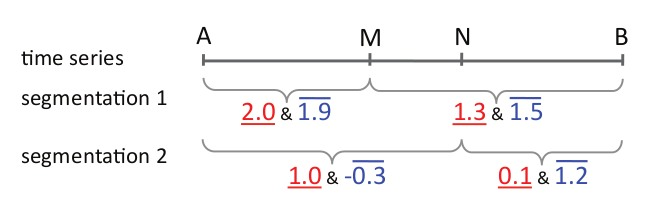
\includegraphics[scale=0.4]{{Images/chap7Hoai}.jpg}}
  \caption{Κατά το σπάσιμο ενός τμήματος ΑΒ έχουμε πολλαπλές επιλογές ως το πλήθος και το μήκος των επιμέρους τμημάτων. Ποια είναι όμως η βέλτιστη; Σύμφωνα με τους Hoai et al. \cite{hoai_2011}, αυτό προκύπτει αναζητώντας το μέγιστο περιθώριο κέρδους μεταξύ της πιο πιθανής κλάσης και της αμέσως λιγότερο πιθανής. Οπότε στην εικόνα του σχήματος, όπου έχουμε δύο κλάσεις με σκορ που φαίνονται στο σχήμα για κάθε τμήμα, προτιμότερο ειναι το σπάσιμο στο σημείο Ν. Εικόνα από \cite{hoai_2011}}
  \label{fig:chap7Hoai}
\end{figure}

\subsection{Εκπαίδευση SVM}
Έστω $n$ το πλήθος βίντεο $X^i$ με $i=1 \dots n$. Για τα βίντεο αυτά είναι γνωστά τα όρια κάθε δράσης, έστω πλήθος $k_i$, στα $0=s_1^i<s_2^i< \dots <s_{k_i+1}^i=len(X^i)$ και αντιστοιχούν στις ετικέτες κλάσεων $y_1^i, \dots, y_{k_i}^i, i=1, \dots, m$. Υπό αυτές τις συνθήκες, στόχος της εκπαίδευσης είναι η ελαχιστοποίηση ως προς $w_i, \xi_t^i \geq 0$ της ποσότητας:

\begin{equation}\label{eq:SVMOpt}
    \frac{1}{2m} \sum_{j=1}^m \| w_i \|^2 +C \sum_{i=1}^n \sum_{t=1}^{k_i} \xi_t^i
\end{equation}

έτσι ώστε να ισχύει

\begin{equation}\label{eq:SVMOptEq}
    (w_{y_t^i}-w_y)^T \phi(X_{(s_t^i,s_{t+1}^i)}^i) \geq 1-\xi_t^i \text{ } \forall i,t,y \neq y_t^i
\end{equation}

όπου $X_{(s_t^i,s_{t+1}^i)}^i$ το τμήμα του βίντεο $X^i$ μεταξύ $[s_t+1,s_{t+1}]$, $\phi(\cdot)$ η συνάρτηση χαρακτηριστικών και $w_y^T \phi(X_{(s_t^i,s_{t+1}^i)}^i)$ τα SVM scores για την ανάθεση του τμήματος αυτού στην κλάση $y$. Ακόμα, στις παραπάνω εξισώσεις χρησιμοποιούνται η παράμετρος $C$ (regularization parameter) που δημιουργεί τις συνθήκες ισορροπίας μεταξύ μεγάλων περιθωρίων κέρδους και ελαφρύτερης παραβίασης των περιορισμών και οι μεταβλητές $\xi_t^i$ (slack variables), που επιτρέπουν μικρή παραβίαση των περιορισμών. Σύμφωνα λοιπόν με αυτή τη σύμβαση, η σχέση \ref{eq:SVMOptEq} απαιτεί το τμήμα να αντιστοιχίζεται στην κλάση $y$ με μεγάλη βεβαιότητα (σχετικά μεγαλύτερο σκορ από κάθε άλλη κλάση για κάποιο περιθώριο κέρδους) και θέλουμε ταυτόχρονα ελαχιστοποίηση των $\xi_t^i$ και των $w_i$, προβλήματα αντιμαχόμενα, οπότε παρέχουμε αντιστάθμιση με την παράμετρο $C$.

\subsection{Κατάτμηση με Καταπίεση μη-Μεγίστων}
Μέσω της εκπαίδευσης έχουμε εξάγει τα βάρη $w_i$. Για την κατάτμηση ζητάμε, για ένα άγνωστο βίντεο $X$, την εύρεση $k$ και ακολουθίας $s_1, \dots s_{k+1}$ έτσι ώστε να ελαχιστοποιείται ως προς $k, s_t, y_t, \xi_t$ η ποσότητα

\begin{equation}\label{eq:SegOpt}
    \sum_{t=1}^k \xi_t
\end{equation}

έτσι ώστε να ισχύει

\begin{equation}\label{eq:SegOptEq}
    l_{min} \leq s_{t+1}-s_t \leq l_{max} \text{ } \forall t \text{ και } (w_{y_t}-w_y)^T \phi(X_{(s_t,s_{t+1})}) \geq 1-\xi_t \text{ } \forall t,y \neq y_t
\end{equation}

με $s_1=0$ και $s_{k+1}=len(X)$, όπου τα $l_{min}, l_{max}$ είναι το ελάχιστο και το μέγιστο μήκος τμήματος αντίστοιχα και υπολογίζονται κατά τη φάση εκπαίδευσης. Η κύρια ιδέα είναι να σπάσουμε το βίντεο έτσι ώστε τα τμήματα να αντιστοιχίζονται σε μία κλάση με μεγάλη βεβαιότητα. Η εξίσωση \ref{eq:SegOpt} απαιτεί να καταπιεστούν οι λιγότερο (μη μέγιστα) πιθανές κλάσεις, αντί να μεγιστοποιεί απευθείας SVM scores.

\subsection{Δυναμικός Προγραμματισμός}
Θεωρούμε τη βέλτιστη κατάτμηση για το τμήμα από 0 ως $u$,

\begin{equation}\label{eq:fOri}
    f(u)=\min_{k,s_t,y_t,\xi_t \geq 0} \sum_{t=1}^k \xi_t
\end{equation}

υπό τους περιορισμούς της εξίσωσης \ref{eq:SegOptEq} μόνο που τώρα $s_{k+1}=u$. Για κάθε συνδυασμό $(u,l)$ με $u \in (0,len(X)), l \in[l_{min},l_{max}]$ ορίζουμε

\begin{equation}\label{eq:ksOri}
    \xi(u,l)=\max \big( 0,1-(w_{\hat{y}}-w_{\tilde{y}})^T \phi(X_{(u-l,u]}) \big)
\end{equation}

με $\hat{y}, \tilde{y}$ τις θέσεις πρώτου και δεύτερου μεγίστου της ποσότητας $w_y^T \phi(X_{(u-l,u]})$. Σκοπός είναι ο υπολογισμός του ελαχίστου $f(len(X))$ με την εξίσωση

\begin{equation}\label{eq:fksOri}
    f(u)=arg\min_l \big( \xi(u,l)+f(u-l) \big)
\end{equation}

η οποία λύνεται με χρήση δυναμικού προγραμματισμού. Η πολυπλοκότητα αυτού του αλγορίθμου είναι $O \big( m (l_{max}-l_{min}+1) len(X) \big)$, δηλαδή $O(n^2)$.


\section{Προτεινόμενος Αλγόριθμος}
Επιχειρηματολογούμε ότι ο αλγόριθμος των \cite{hoai_2011} έχει ένα σαφές μειονέκτημα σε σύνολα δεδομένων τα οποία ενσωματώνουν την κατηγορία δράσεων υποβάθρου στις κλάσεις τους: επιβραβεύει την κατάτμηση σε μεγάλα τμήματα τα οποία κατατάσσονται στην κλάση δράσεων υποβάθρου. Πράγματι, ο αλγόριθμος επιχειρεί να ελαχιστοποιήσει ένα άθροισμα, άρα μια μη φραγμένη ποσότητα. Δεδομένου ότι οι όροι που αθροίζονται είναι όλοι μη αρνητικοί, το άθροισμα επιβαρύνεται με τη σώρρευση πολλών μικρών τμημάτων. Αντίθετα, ένα τμήμα που περιλαμβάνει πολλές μικρές ενέργειες, μπορεί να ταξινομηθεί συνολικά ως δράση υποβάθρου. Αυτό βέβαια εξαρτάται και από τη δύναμη του ταξινομητή, αλλά μόνο ιδανικά ο ταξινομητής θα επιβραβεύει με θριαμβευτικά μεγάλο κέρδος την πιο πιθανή κλάση. Επιπλέον, το κόστος του αλγορίθμου είναι αρκετό, ειδικά όταν η εξαγωγή των χαρακτηριστικών τμήματων είναι βαριά.

\par Προτείνουμε λοιπόν τον εξής αλγόριθμο, ο οποίος βελτιώνει αυτόν των \cite{hoai_2011}. Σε πρώτη φάση, θεωρώντας την ακολουθία αντικειμένων (ή γενικότερα λεξιλογίου) ως ισχυρό χαρακτηριστικό αναγνώρισης δράσεων, τεμαχίζουμε το βίντεο σε τμήματα στα οποία το διάνυσμα αντικειμένων παραμένει σταθερό. Δηλαδή, ορίζουμε τα τμήματα των δράσεων ως τα σημεία διαφοροποίησης των αντικειμένων που παρατηρούμε. Στη συνέχεια εφαρμόζουμε έναν αλγόριθμο δυναμικού προγραμματισμού, ο οποίος επιβραβεύει τη μέγιστη βεβαιότητα των τμημάτων, αντί για τη μέγιστη συνολική βεβαιότητα θραύσης. Συγκεκριμένα, σε κάθε τμήμα με σταθερό διάνυσμα αντικειμένων, εξετάζουμε όλα τα πιθανά συμπληρωματικά υποτμήματα, 2 σε πλήθος, που αν ενωθούν σε συνθετουν το βίντεο. Δηλαδή, σπάμε το υποτμήμα σε δύο μικρότερα με όλους τους δυνατούς τρόπους. Έστω μια θέση $u$ μες στο υποτμήμα. Αριθμούμε για ευκολία τις θέσεις αυτές από 0 ως $len(X_i)$, για το υποτμήμα $X_i$. Τότε ζητάμε το $u$ που ελαχιστοποιεί την ποσότητα

\begin{equation}\label{eq:fksOriD}
\begin{gathered}
    f(u)=min(\big( \xi(u,u), \xi(len(X_i),len(X_i)-u) \big) \\ =min\big( \max \big( 0,1-(w_{\hat{y}}-w_{\tilde{y}})^T \phi(X_{(0,u]}) \big), \max \big( 0,1-(w_{\hat{y}}-w_{\tilde{y}})^T \phi(X_{(u,len(X_i)]}) \big) \big)
\end{gathered}
\end{equation}

Προσεγγίζουμε την ποσότητα $(w_{\hat{y}}-w_{\tilde{y}})^T \phi(X_{(u-l,u]})$ με τις αντίστοιχες πιθανότητες για τις δύο πιο πιθανές κλάσεις, οπότε η ποσότητα αυτή γράφεται ισοδύναμα $\Delta P_{(u-l,u]}$, που πρόκειται για μια μη αρνητική ποσότητα μικρότερη ή ίση του 1. Άρα η παραπάνω σχέση \ref{eq:fksOriD} γράφεται τώρα

\begin{equation}\label{eq:fksOriD2}
    f(u)=min\big( 1-\Delta P_{(0,u]} , 1-\Delta P_{(u,len(X_i)]} \big)
\end{equation}

Είναι φανερό ότι από τα δύο τμήματα που τελικά θα προκύψουν, το ένα δεν θα δέχεται επιπλέον σπάσιμο, αφού έχει επιτευχθεί το ελάχιστο σκορ. Οπότε τρέχουμε τον ίδιο αλγόριθμο στο δεύτερο τμήμα. Σταματάμε τις επαναλήψεις όταν ένα υποτμήμα ταξινομηθεί ολόκληρο με βέλτιστο σκορ. Στο σημείο αυτό αναφέρουμε ότι στα άκρα πρέπει να ισχύει μια διαφορετική συνθήκη. Όταν εξετάζουμε ένα τμήμα ως σύνολο τότε αποδίδουμε για τη θέση αυτή σκορ ίσο με το σκορ του τμήματος. Δηλαδή αποδίδουμε άπειρο σκορ σε τμήμα μηδενικού μήκους. Τέλος, συγχωνεύουμε διαδοχικά τμήματα που έχουν ταξινομηθεί στην ίδια κλάση.

\par Από άποψη πολυπλοκότητας, ο αλγόριθμος εκκινεί σπάζοντας το βίντεο σε κομμάτια, τάξης $O(1)$. Σε κάθε τμήμα μήκους $l$, διατρέχουμε $l$ υπολογισμούς για να βρούμε το ελάχιστο σκορ και στη συνέχεια σπάμε το τμήμα και διατρέχουμε μόνο το ένα θραύσμα. Γίνεται φανερό ότι ο αλγόριθμος εντός ενός τμήματος είναι στην καλύτερη περίπτωση $O(n)$ (το τμήμα ταξινομείται ενιαία βέλτιστα), στη μέση περίπτωση $O(nlogn)$ (σπάμε σε $O(logn)$ κομμάτια για τα οποία εκτελούμε $O(n)$ υπολογισμούς) και στη χειρότερη περίπτωση $O(n^2)$ (τα βέλτιστα τμήματα είναι πολυ μικρού μήκους και πρακτικά περνάμε ολόκληρο το τμήμα πολλές φορές). Δεδομένου ότι τα θραύσματα είναι της τάξης $O(1)$, ο συνολικός αλγόριθμος έχει μέση πολυπλοκότητα $O(nlogn)$. Το γεγονός αυτό καθιστά τον αλγόριθμο αρκετά πιο αποδοτικό από τον προτεινόμενο των \cite{hoai_2011}.

\par Παρουσιάζουμε εδώ τα δομικά μέρη της παραπάνω λογικής διαδικασίας. Ο αλγόριθμός μας εκκινεί από την κατάτμηση του βίντεο με βάση τις αλλαγές στα εμφανιζόμενα αντικείμενα. Με κάποια απλότητα, δείχνουμε εδώ μια τέτοια συνάρτηση:

\begin{algorithm}[H]
	\caption{Πρώτη φάση του προτεινόμενου αλγορίθμου: κατάτμηση του βίντεο σύμφωνα με τα σημεία μεταβολής των εμφανίσεων αντικειμένων}
	\label{alg:ObjSeg}
	\begin{algorithmic}
	  \Function{ObjectSegmentation}{$video$}
	  \State $objectSegments$=[]
	  \For {$f=1:length(frames)$}\\
		\If {$objectFeatures(f,:) \neq objectFeatures(f-1,:)$}
		  \State $concatenate(objectSegments, f)$
		\EndIf
	  \EndFor
	  \State \Return $objectSegments$
	  \EndFunction
	\end{algorithmic}
\end{algorithm}

\par Έχοντας λάβει τα αρχικά τμήματα, αναλύουμε το κάθε ένα από αυτά ξεχωριστά εφαρμόζοντας μια μέθοδο δυναμικού προγραμματισμού. Συνενώνουμε τα επιμέρους τμήματα που προκύπτουν και έχουμε το σύνολο των θραυσμάτων. Ένα βήμα που δε φαίνεται στον παρακάτω αλγόριθμο είναι η συνένωση διαδοχικών τμημάτων με ίδια ετικέτα κλάσης. Όπου στους παρακάτω αλγορίθμους φαίνεται ως όρισμα συνάρτησης ένα διάστημα της μορφής $[A,B)$, αυτό αφορά όλους τους ακεραίους από το Α (συμπεριλαμβανομένου του Α), μέχρι το Β (μη συμπεριλαμβάνοντας το Β).

\begin{algorithm}[H]
	\caption{Κύριος κορμός του προτεινόμενου αλγορίθμου: κλήση της συνάρτησης δυναμικού προγραμματισμού για κάθε τμήμα βίντεο που έχει προκύψει από το σπάσιμο σύμφωνα με τις μεταβολές αντικειμένων και σώρρευση των αποτελεσμάτων. Τα αποτελέσματα λαμβάνονται από τις λίστες FinalClassification και FinalSegmentation.}
	\label{alg:MainSeg}
	\begin{algorithmic}
	  \Function{CoreSegmentation}{$video$}
	  \State $FinalSegmentation=[]$ \Comment{start frames of computed segments}
	  \State $FinalClassification=[]$ \Comment{classes of computed segments}
	  \State $objectSegments$=\Call{ObjectSegmentation}{$video$}
	  \For {$s=2:length(objectSegments)$}
		\State $finalSegments,finalClasses$=\Call{DynamicSegmentation}{$[objectSegments(s-1), objectSegments(s))$}
		\State $concatenate(FinalSegmentation, finalSegments)$
		\State $concatenate(FinalClassification, finalClasses)$
	  \EndFor
	  \EndFunction
	\end{algorithmic}
\end{algorithm}

\par Ο πυρήνας της συνάρτησης δυναμικού προγραμματισμού φαίνεται αμέσως παρακάτω. Αφού εξαχθούν τα χαρακτηριστικά και υπολογιστεί η SVM Loss με χρήση των πιθανοτήτων των δύο πιθανότερων κλάσεων, αντιπροσωπεύουμε έναν συνδυασμό τμημάτων, δηλαδή μια τομή, με την ελάχιστη των δύο πιθανοτήτων για τα τμήματα. Κρατάμε την τομή με το ελάχιστο κόστος και ορίζουμε ως πιθανό εσωτερικό σημείο θραύσης την τομή αυτή. Το τμήμα με την ελάχιστη πιθανότητα έχει πλέον ταξινομηθεί βέλτιστα και τρέχουμε την ίδια συνάρτηση για το δεύτερο τμήμα.

\begin{algorithm}[H]
	\caption{Συνάρτηση Δυναμικού Προγραμματισμού για την επαναληπτική κατάτμηση ενός δοθέντος τμήματος με σταθερές επισημειώσεις αντικειμένων.}
	\label{alg:Dynamic}
	\begin{algorithmic}
	  \Function{DynamicSegmentation}{$segment$}
	  \State $[Loss, Classes, Segments]=$ \Call{ProbabilityComputation}{$segment$}
	  \State $segmentStart=argmin(Loss)$
	  \State $segmentClass=Classes(segmentStart)$
	  \If $segmentStart==1$
		$finalSegments=segment(segmentStart)$
		$finalClassses=segmentClass$
	  \ElsIf {$Segments(segmentStart)==1$}
		  \State $newFinalSegments, newFinalClasses=$ \Call{dynamicSegmentation}{$[segment(segmentStart), segment(end))$}
		  \State $finalSegments=concatenate(segment(segmentStart), newFinalSegments)$
		  \State $finalClasses=concatenate(segmentClass, newFinalClasses)$
	  \Else
		  \State $newFinalSegments, newFinalClasses=$ \Call{dynamicSegmentation}{$[segment(segmentStart), segment(end))$}
		  \State $finalSegments=concatenate(newFinalSegments, segment(segmentStart))$
		  \State $finalClasses=concatenate(newFinalClasses, segmentClass)$
	  \EndIf
	  \Return {$finalSegments, finalClasses$}
	  \EndFunction
	\end{algorithmic}
\end{algorithm}

\par Ο υπολογισμός των πιθανοτήτων απαιτεί τον υπολογισμό τους και την διαμόρφωσή τους από την πληροφορία κειμένου. Σε πρώτη φάση εξάγονται τα χαρακτηριστικά για το κάθε τμήμα βίντεο. Γίνεται ταξινόμηση για κάθε ένα από αυτά και υπολογίζουμε την SVM Loss με χρήση πιθανοτήτων, όπως περιγράφηκε νωρίτερα. Επιστρέφουμε την τιμή της SVM Loss για κάθε τμήμα, την προκύπτουσα κλάση στην οποία ταξινομείται και το υποτμήμα του (πρώτο ή δεύτερο) στο οποίο αντιστοιχεί η τιμή SVM Loss αυτή.

\begin{algorithm}[H]
	\caption{Αλγόριθμος εξαγωγής SVM Loss και κλάσεων μέσω πιθανοτήτων. Χωρίζουμε κάθε πιθανό τμήμα σε Left και Right, τα οποία δείχνουν το πώς το αρχικό τμήμα έχει σπάσει σε δύο.}
	\label{alg:Probs}
	\begin{algorithmic}
	  \Function{ProbabilityComputation}{$segment$}
	  \For {$s=1:length(segment)$}
		\State $featuresLeft=$ \Call{extractFeatures}{$[segment(1), segment(s))$}
		\State $featuresRight=$ \Call{extractFeatures}{$[segment(s), segments(end))$}
		\State $probabilitiesLeft=$ \Call{classify}{$featuresLeft$}
		\State $probabilitiesRight=$ \Call{classify}{$featuresRight$}
		\State $sortedPLeft=sort(probabilitiesLeft)$
		\State $sortedPRight=sort(probabilitiesRight)$
		\State $lossLeft=1-(sortedPLeft(1)-sortedPLeft(2))$
		\State $lossRight=1-(sortedPRight(1)-sortedPRight(2))$
		\State $classLeft=argmin(probabilitiesLeft)$
		\State $classRight=argmin(probabilitiesRight)$
		\State $Loss(s)=min(lossLeft,lossRight)$
		\State $Segments(s)=argmin(lossLeft, lossRight)$
		\State $classes=concatenate(classLeft, classRight)$
		\State $Classes(s)=classes(Segments(s))$
	  \EndFor
	  \Return{$Loss, Classes, Segments$}
	  \EndFunction
	\end{algorithmic}
\end{algorithm}

\par Τρέξαμε τον αλγόριθμο κατάτμησης σε 18 από τα 20 test βίντεο, λόγω περιορισμών υπολογιστικών πόρων σε θέματα μνήμης. Για την αξιολόγηση των αποτελεσμάτων χρησιμοποιούμε τη μετρική Mean Average Precision που περιγράψαμε στο προηγούμενο κεφάλαιο, ελέγχοντας την μετρική ανά frame βίντεο. Σε 323262 test frames, \textbf{ο αλγόριθμός μας πιάνει απόδοση 46.4\% mAP}. Καθώς, από όσο γνωρίζουμε δεν έχουν δημοσιευτεί αποτελέσματα κατάτμησης δράσεων για το συγκεκριμένο σύνολο δεδομένων, δεν μπορούμε να συγκρίνουμε αυτό το αποτέλεσμα με άλλα της βιβλιογραφίας.

\par Το πλήθος των δράσεων που αναγνωρίζουμε (61) και το μεγάλο μήκος των βίντεο σε frames (18000 frames κατά μέσο όρο) αποτρέπουν μια λεπτομερή οπτικοποίηση των αποτελεσμάτων στο χρονικό ορίζοντα. Αντί αυτού, παραθέτουμε μια ένδειξη της απόδοσης του αλγορίθμου στο πρόβλημα της κατάτμησης σε δράσεις ή υπόβαθρο. Πρόκειται για ένα δυαδικό πρόβλημα το οποίο είναι ενδιαφέρον λόγω της ανισορροπίας του πλήθους των δειγμάτων των κλάσεων. Πιο αναλυτικά, η κλάση υποβάθρου καταλαμβάνει το 35\% περίπου των δειγμάτων εκπαίδευσης, ποσοστό υπερβολικά μεγαλύτερο από το αντίστοιχο όλων των υπολοίπων κλάσεων. Επομένως αναμένουμε η κλάση αυτή να εμφανίζεται αρκετά συχνά και στα test videos, οπότε η ικανότητα διαχωρισμού των δράσεων υποβάθρου από τις υπόλοιπες είναι σημαντικό ζήτημα. Ως μεμονωμένο πείραμα, μετρήσαμε την μετρική mAP για το δυαδικό πρόβλημα υπόβαθρο ή μη υπόβαθρο και βρήκαμε 80.5\% mAP. Το σχήμα \ref{fig:segmentation19} δείχνει τα αποτελέσματα αυτής της διάκρισης σε ένα βίντεο ελέγχου.

\begin{figure}
  \centering
  \noindent\makebox[\textwidth]{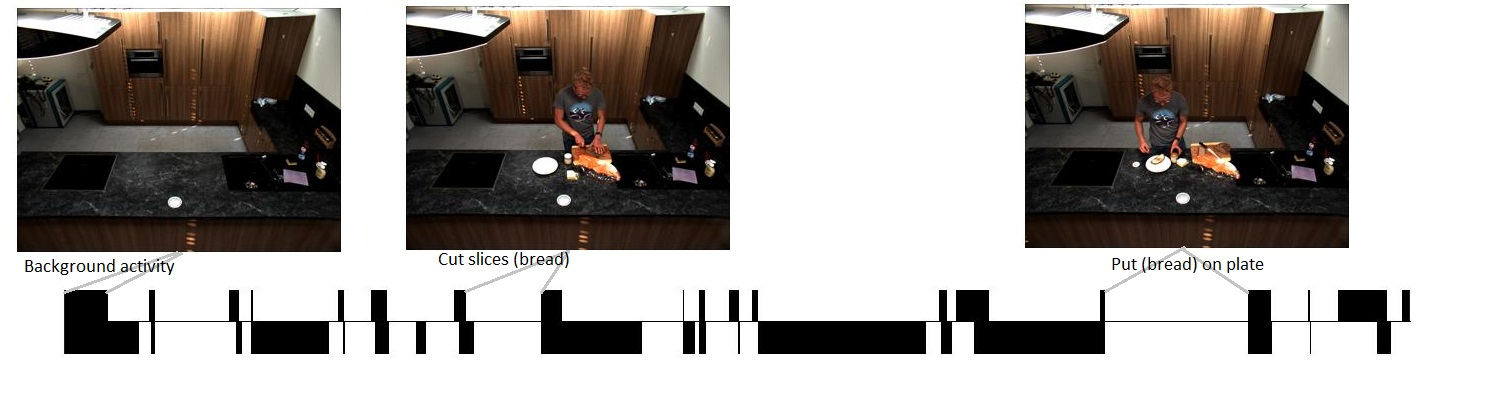
\includegraphics[scale=0.5]{{Images/segmentation19}.jpg}}
  \caption{Αποτελέσματα της κατάτμησης του βίντεο s19-d01 για το δυαδικό πρόβλημα δράσεων υποβάθρου εναντίον δράσεων μη υποβάθρου. Ποιοτικά (εικόνα) αλλά και ποσοτικά (80.5\% mAP) τα αποτελέσματα είναι ικανοποιητικά. Η παρούσα εικόνα δείχνει \textbf{με μαύρο τις περιοχές δράσεων υποβάθρου και με λευκό τις δράσεις προσκηνίου}. Όπως φαίνεται, το σχήμα περικλείει δύο γραμμες αποτελεσμάτων. \textbf{Στην πάνω γραμμή φαίνεται η πραγματική (ground truth) κατάτμηση και στην κάτω η υπολογισμένη κατάτμηση με χρήση του αλγορίθμου που προτείνουμε.}}
  \label{fig:segmentation19}
\end{figure}

\end{document}
